\documentclass[twocolumn]{article}
\usepackage[utf8]{inputenc}
\usepackage[T1]{fontenc}
\usepackage[spanish]{babel}
\usepackage[spanish]{translator}
\usepackage{amsmath}
\usepackage{graphicx}
\usepackage{booktabs}
\usepackage{float}
\usepackage{hyperref}

\title{Simulación de la Precesión del Perihelio de Mercurio}
\author{Brian David Leiva. ECFM - USAC}
\date{Noviembre, 2024}

\begin{document}

\maketitle

\begin{abstract}
Este estudio investiga la precesión del perihelio de Mercurio utilizando métodos numéricos, específicamente el método de Runge-Kutta de segundo orden (RK2). Se desarrolla un modelo computacional que incorpora tanto la fuerza gravitacional del Sol como los efectos perturbadores de otros planetas y correcciones relativistas representados por un parámetro $\alpha$. El trabajo comienza con una introducción a los métodos de Runge-Kutta y una descripción detallada de la órbita de Mercurio, incluyendo las ecuaciones que gobiernan su movimiento.
\end{abstract}
\section{Introducción}

\subsection*{Métodos de Runge-Kutta}

Los métodos de Runge-Kutta son una familia de algoritmos numéricos iterativos utilizados para aproximar soluciones de ecuaciones diferenciales ordinarias (EDOs). Estos métodos son ampliamente utilizados en física computacional y otras disciplinas científicas.

Los métodos de Runge-Kutta funcionan calculando incrementos intermedios entre cada paso de integración, lo que permite una mejor aproximación de la solución real. Para este estudio, utilizaremos el método de Runge-Kutta de segundo orden (RK2). Este método ofrece un buen equilibrio entre precisión y eficiencia computacional para nuestro problema.

La fórmula general para el método RK2 es:

\begin{equation}
y_{n+1} = y_n + k_2
\end{equation}

Donde:
\begin{itemize}
\item $y_n$ es el valor actual de la función
\item $\Delta t$ es el tamaño del paso
\item $k_1 = \Delta t \cdot f(t_n, y_n)$
\item $k_2 = \Delta t \cdot f(t_n + \Delta t/2, y_n + k_1/2)$
\end{itemize}

En el caso de la órbita de Mercurio, el método RK2 nos permite resolver numéricamente las ecuaciones de movimiento derivadas de la fuerza gravitacional.

La aplicación del método RK2 a este problema implica descomponer las ecuaciones de movimiento en un sistema de ecuaciones diferenciales de primer orden y luego aplicar el algoritmo iterativamente para avanzar la posición y velocidad de Mercurio en el tiempo. Aunque el RK2 es menos preciso que métodos de orden superior como el RK4, es suficiente para nuestro estudio.

\subsection*{La órbita de Mercurio}

Para modelar con precisión el movimiento de Mercurio, es necesario considerar no solo la fuerza gravitatoria del Sol, sino también los efectos de otros planetas y efectos relativistas.

La ecuación para la fuerza gravitatoria sobre Mercurio, que incluye las correcciones relativistas y el efecto gravitatorio de otros planetas como una fuerza externa, se puede expresar de la siguiente manera \cite{chang}:

\begin{equation}
F =  \frac{G M_s M_m }{r^2}(1 + \frac{\alpha}{r^2})
\end{equation}

Donde:
\begin{itemize}
\item $F$ es la fuerza gravitatoria
\item $G$ es la constante de gravitación universal
\item $M_s$ es la masa del Sol
\item $M_m$ es la masa de Mercurio
\item $r$ es la distancia entre el centro del Sol y el centro de Mercurio
\item $\alpha$ es un parámetro que representas las correcciones mencionadas.
\end{itemize}

\section{Metodología}
\subsection*{Aplicando los métodos de Runge-Kutta a la órbita de Mercurio}

Para aplicar el método de Runge-Kutta de segundo orden (RK2) a la órbita de Mercurio, necesitamos primero expresar las ecuaciones de movimiento en un sistema de ecuaciones diferenciales de primer orden.

Partiendo de la fuerza gravitatoria que actúa sobre Mercurio:

\begin{equation}
F =  \frac{G M_s M_m }{r^2}(1 + \frac{\alpha}{r^2})
\end{equation}

Podemos expresar las ecuaciones de movimiento en coordenadas polares $(r, \theta)$ de la siguiente manera:

\begin{equation}
\frac{d^2r}{dt^2} - r \cdot \left(\frac{d\theta}{dt}\right)^2 = -G \cdot M_s \cdot \frac{1}{r^2} \cdot (1 + \frac{\alpha}{r^2})
\end{equation}

\begin{equation}
\frac{1}{r} \cdot \frac{d}{dt}\left(r^2 \cdot \frac{d\theta}{dt}\right) = 0
\end{equation}

Para aplicar el método RK2, necesitamos convertir estas ecuaciones de segundo orden en un sistema de ecuaciones de primer orden. Definimos las siguientes variables:

\begin{itemize}
\item $u = r$
\item $v = \frac{dr}{dt}$
\item $w = \frac{d\theta}{dt}$
\end{itemize}

Ahora, podemos reescribir nuestras ecuaciones como un sistema de primer orden:

\begin{equation}
\frac{du}{dt} = v
\end{equation}

\begin{equation}
\frac{dv}{dt} = u \cdot w^2 - \frac{G \cdot M_s}{u^2} \cdot (1 + \frac{\alpha}{u^2})
\end{equation}

\begin{equation}
\frac{dw}{dt} = -\frac{2v \cdot w}{u}
\end{equation}

Este sistema de ecuaciones diferenciales de primer orden es el que resolveremos utilizando el método RK2. En cada paso de tiempo, aplicaremos el algoritmo RK2 a cada una de estas ecuaciones para actualizar los valores de $u$, $v$, y $w$, que representan la posición radial, la velocidad radial y la velocidad angular de Mercurio, respectivamente.

\subsection*{Implementando una función de iteración}

Implementamos la función \texttt{simular\_orbita\_mercurio} en Python, la cual simula la órbita de Mercurio utilizando el método de Runge-Kutta de segundo orden (RK2). Esta función toma los siguientes parámetros:

\begin{itemize}
    \item \texttt{x\_inicial} (float, opcional): Posición inicial en el eje x. Si no se proporciona, se calcula como $(1+e)a$, donde $e$ es la excentricidad y $a$ es el semieje mayor de la órbita.
    \item \texttt{y\_inicial} (float, opcional): Posición inicial en el eje y. Por defecto es 0.
    \item \texttt{vx\_inicial} (float, opcional): Velocidad inicial en el eje x. Por defecto es 0.
    \item \texttt{vy\_inicial} (float, opcional): Velocidad inicial en el eje y. Si no se proporciona, se calcula utilizando la ecuación de la velocidad orbital.
    \item \texttt{iteraciones} (int, opcional): Número de iteraciones para la simulación. Por defecto es 20000.
    \item \texttt{delta\_t} (float, opcional): Tamaño del paso de tiempo para la simulación. Por defecto es 0.0001.
    \item \texttt{alpha} (float, opcional): Parámetro que representa la corrección relativista. Por defecto es 0.0008.
\end{itemize}

La función inicializa las variables necesarias, incluyendo constantes como $GM_s$ para representar la gravedad del sol, el semieje mayor ($a$), y la excentricidad ($e$) de la órbita de Mercurio.

Luego, realiza la simulación utilizando el método RK2, calculando en cada iteración:
\begin{enumerate}
    \item Las variables radiales y totales ($r$ y $v$).
    \item Los valores intermedios ($k_1$) para posición y velocidad.
    \item Los valores finales ($k_2$) para posición y velocidad.
    \item Actualiza los valores de posición, velocidad y tiempo para el siguiente paso.
\end{enumerate}

La función devuelve tres listas:
\begin{enumerate}
    \item \texttt{tiempos}: Una lista con los tiempos de cada paso de la simulación.
    \item \texttt{posiciones}: Una lista de tuplas $(x, y)$ representando las posiciones en cada paso.
    \item \texttt{velocidades}: Una lista de tuplas $(v_x, v_y)$ representando las velocidades en cada paso.
\end{enumerate}

Esta implementación nos permite simular la órbita de Mercurio con diferentes parámetros iniciales y observar cómo estos afectan la precesión del perihelio.

\subsection*{Encontrando la precesión para un $\alpha$ dado}

Para analizar la precesión del perihelio de Mercurio, graficamos la relación entre el parámetro $\alpha$ y el ángulo de la posición con respecto al eje x en el perihelio. Esto nos permite visualizar cómo el parámetro $\alpha$ afecta a la precesión de la órbita.

Luego implementamos una función \texttt{calcular\_precesion} para determinar la precesión del perihelio basados en los resultados de una simulación. Esta función realiza los siguientes pasos:

\begin{enumerate}
    \item Identifica los puntos de perihelio en la órbita simulada. Estos son los puntos donde la distancia al Sol es mínima en cada revolución. Utilizamos dos criterios para identificar los mínimos:
    Son aquellos puntos que son menores que sus dos vecinos y que al mismo timepo son los puntos donde la razón de cambio de la distancia radial se desvanece:
    \begin{equation}
    \frac{dr}{dt} = \frac{xv_x + yv_y}{r} = 0
    \end{equation}
     \item Para cada perihelio se calcula el ángulo de la posición con respecto al eje x. La razón de cambio de este ángulo con respecto al tiempo es la precesión buscada.
\end{enumerate}

\subsection*{Extrapolando el valor de la Precesión para un Valor de $\alpha$ Difícil de simular}

Una vez que tenemos la función \texttt{calcular\_precesion} podemos utilizarla para simular la órbita de Mercurio para diferentes valores de $\alpha$, y luego encontrar la pendiente de la recta que relaciona el parámetro $\alpha$ con la precesión. Esto nos permite extrapolar el valor de la precesión cuando $\alpha = 1.1 \times 10^{-8}$, el cual es difícil de simular dado que tomaría mucho tiempo observar la precesión.


\section{Resultados}

\begin{figure}[H]
\centering
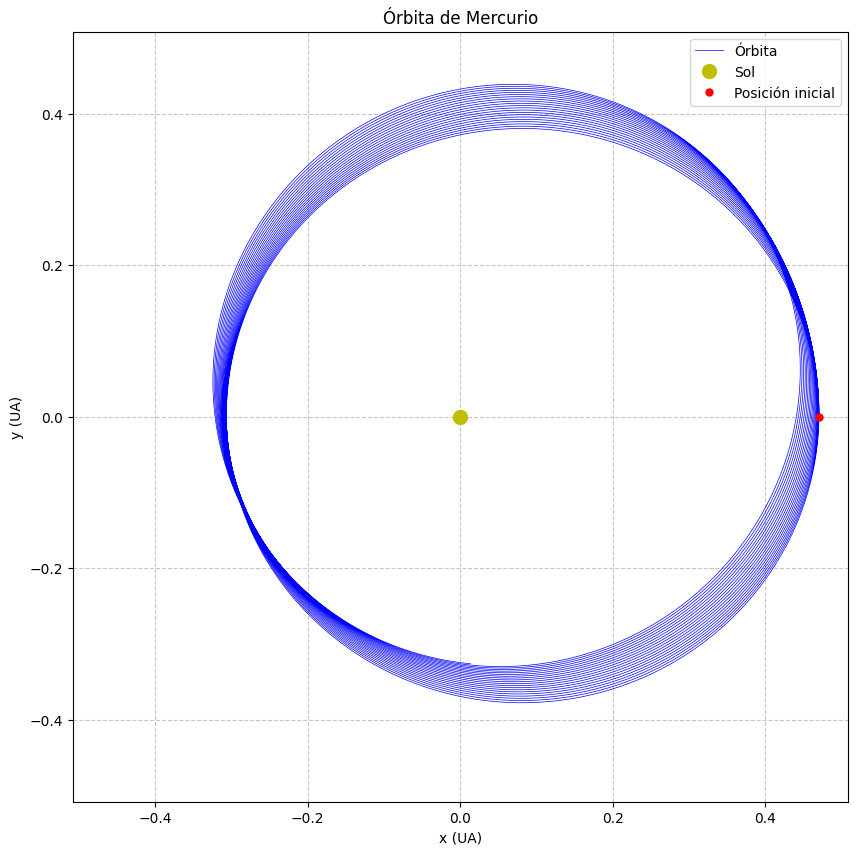
\includegraphics[width=0.9\columnwidth]{./figures/orbita_mercurio.png}
\caption{Órbita simulada de Mercurio}
\label{fig:orbita}
\end{figure}

La Figura \ref{fig:orbita} muestra la órbita simulada de Mercurio utilizando nuestro método de Runge-Kutta de segundo orden. Como se puede observar, la órbita presenta una forma elíptica característica, con el Sol ubicado en uno de los focos de la elipse.

\begin{figure}[H]
\centering
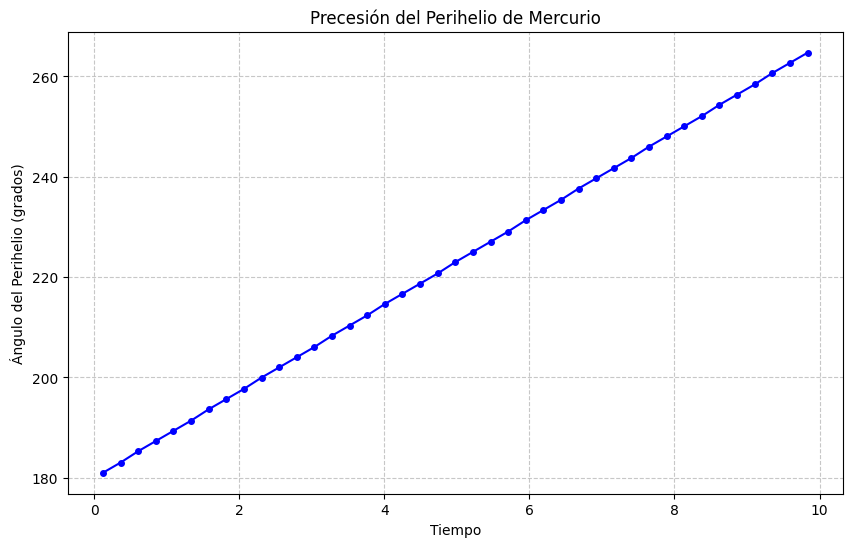
\includegraphics[width=0.9\columnwidth]{./figures/precesion_mercurio.png}
\caption{Ángulo vs. Tiempo para la órbita de Mercurio}
\label{fig:angulo_vs_tiempo}
\end{figure}

En la Figura \ref{fig:angulo_vs_tiempo} podemos observar la relación lineal entre el ángulo y el tiempo, lo que nos permite reconocer la precesión del ángulo como la razón de cambio del ángulo con respecto al tiempo, es decir la pendiente de la recta trazada por el ángulo.

Finalmente, la Tabla \ref{tab:precesion} muestra la precesión calculada para los valores de $\alpha$ requeridos (0.0008, 0.001, 0.002, 0.004) basados en los cuales podemos encontrar la pendiente de 10848.00 para la recta que relaciona $\alpha$ con la precesión. Por lo que para $\alpha = 1.1 \times 10^{-8}$ observado tendríamos una precesión de 42.96 segundos de arco por siglo.

\begin{table}[H]
\centering
\caption{Precesión calculada para diferentes valores de $\alpha$}
\label{tab:precesion}
\begin{tabular}{@{}cc@{}}
\toprule
$\alpha$ & Precesión ($\frac{d\theta}{dt}$) \\
\midrule
0.0008 & 8.63 \\
0.001 & 10.80 \\
0.002 & 22.1 \\
0.004 & 46.41 \\
\bottomrule
\end{tabular}
\end{table}

\section{Discusión}

Notemos que este valor de 42.96 segundos por siglo es lo que se obtiene luego de convertir la precesión devuelta por nuestro código en grados por año. Los detalles se pueden ver en el notebook \cite{mercury_notebook}, donde la conversión es explícita.

\begin{figure}[H]
\centering
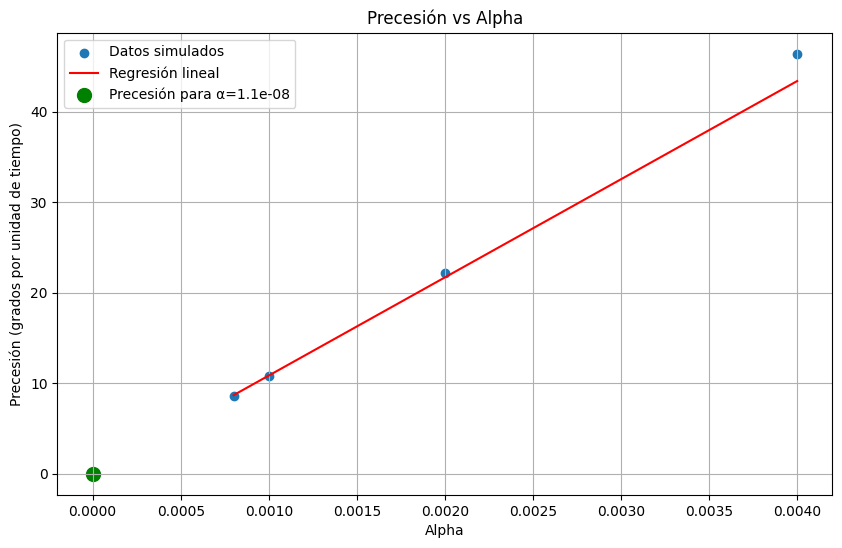
\includegraphics[width=0.9\columnwidth]{./figures/precesion_vs_alpha_mercurio.png}
\caption{Precesión vs. $\alpha$ para la órbita de Mercurio}
\label{fig:precesion}
\end{figure}

El cálculo de la pendiente que relaciona la precesión con el parámetro $\alpha$ se hizo tomando en cuenta los dos primeros puntos de la lista, dado que es una relación lineal, utilizar métodos más avanzados no nos mostraba ninguna mejora en el valor de la precesión. Peor aún, dado que al aumentar $\alpha$, la órbita se aleja cada vez más de los valores observados, los puntos con $\alpha = 0.002, 0.004$ tienden a exagerar más la precesión, como se puede observar al comparar la línea de tendencia lineal en la Figura \ref{fig:precesion} con los valores de la simulación.

\section{Conclusiones}

Fuimos capaces de implementar la función \texttt{simular\_orbita\_mercurio} y verificar el correcto funcionamiento de la simulación. Utilizando esta función pudimos encontrar la relación entre el parámetro $\alpha$ de corrección relativista y la precesión de la órbita. Verificando así nuestra implementación del algoritmo RK2.

\begin{thebibliography}{3}

\bibitem{chang}
Chang, J. D. (2023). Física Computacional. 
\url{https://drive.google.com/file/d/1QOEGPR-jIpCUedNI7W8OMfSFOAApqNSS/view}

\bibitem{github_repo}
Leiva, B. (2023). Física Computacional GitHub Repository. 
\url{https://github.com/BrianDL/fisica_computacional/tree/main}

\bibitem{mercury_notebook}
Leiva, B. (2023). Simulación de la Órbita de Mercurio - Jupyter Notebook. 
\url{https://github.com/BrianDL/fisica_computacional/blob/main/2%20-%20Perihelio%20de%20Mercurio/simulacion_mercurio.ipynb}

\end{thebibliography}

\end{document}